\section{Evaluation} \label{sec:evaluation}
\todo[inline, color=red]{Britta}

\subsection{Tasks} \label{sec:tasks}
\todo[inline, color=yellow]{Anna}
In the supermarket are four different tasks the user has to do. In every tasks a object has to be selected and placed on a target area. If the correct object is placed, the target area will change the color to signal that the tasks is successful done. In the script \textit{TargetTest.cs}, which will be a component of the target object, will be recognized when the target object hits the target area. At this moment the texture of target area will be changed and the measurement will be stopped. More information about the measurement will be mentioned in section \ref{sec:measurement}.\\
In the first three tasks the user has to select different objects. In this tasks the user decides which methods he/she uses. The selected methods should differ depending on the tasks. In these tasks objects far away as well as closely should be picked. \\
The tasks will be shown on the controller similar to the selfteaching which the user is already aware of, shown in the following figure. 

\begin{figure}[H] 
	\center 
	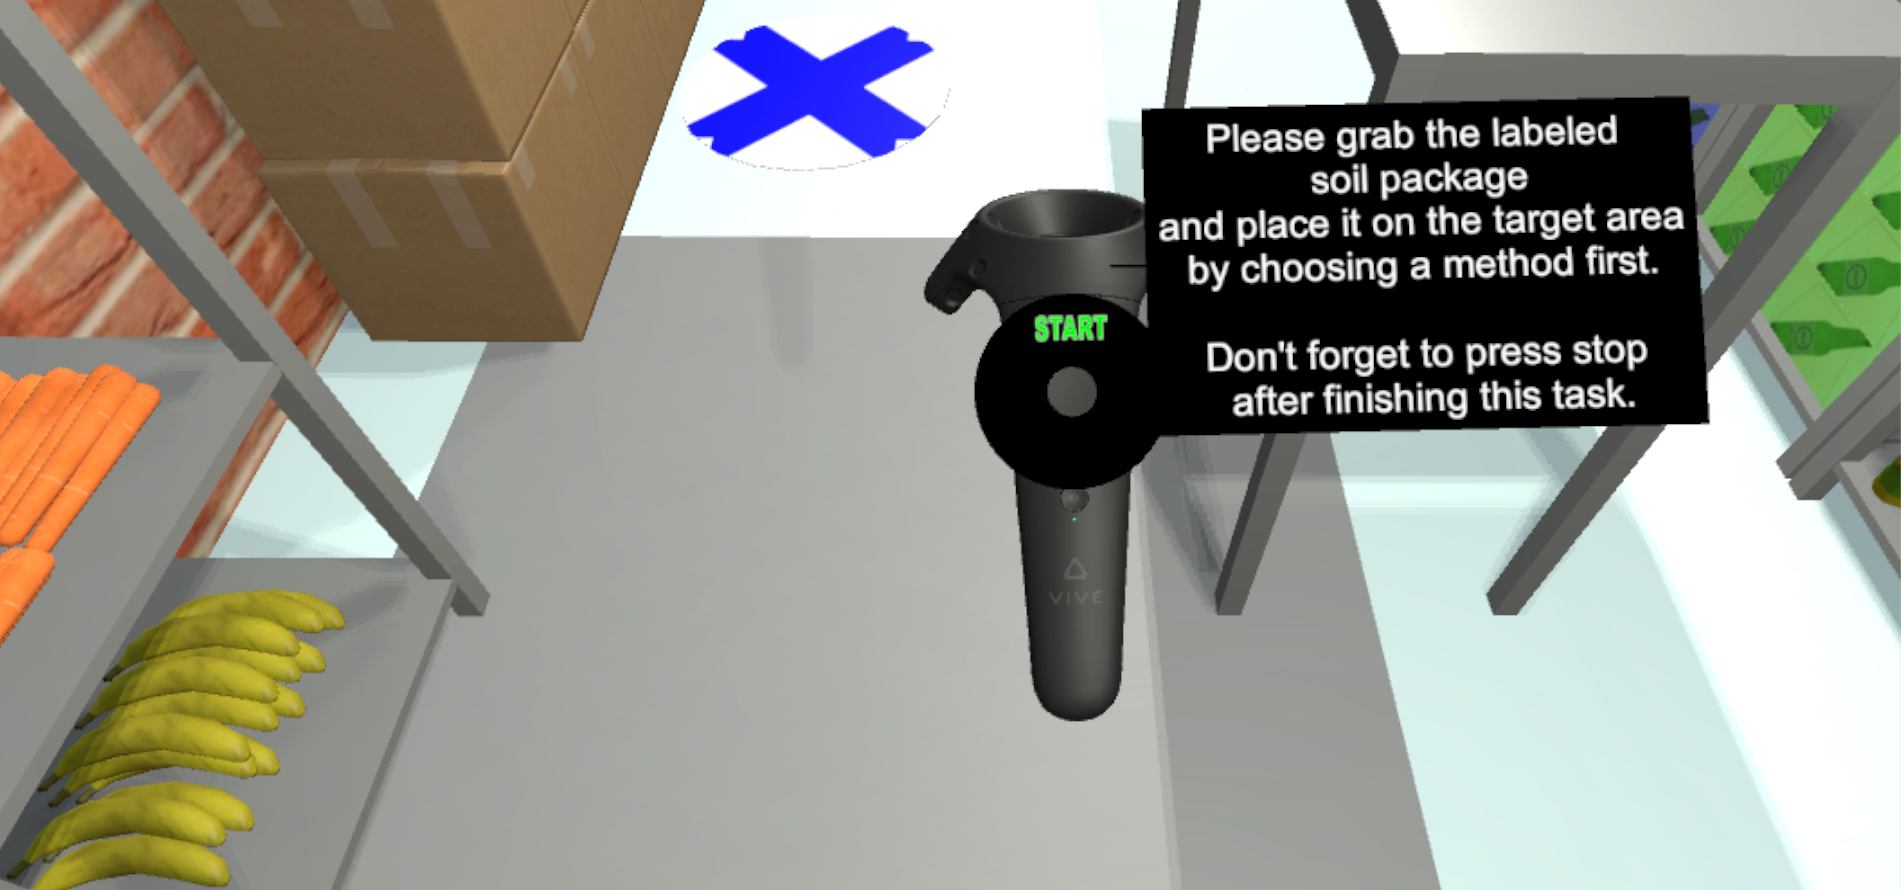
\includegraphics[width=12cm]{Images/TaskContreoller.PNG}
	\caption[Task shown on the controller]{Task shown on the controller}
	\label{fig:taskC}
\end{figure} 

The text for the tasks are saved in a CSV-file, similar to the selfteaching, see section \ref{sec:selfteaching}. The implementation is also related to the selfteaching and implemented in the script \textit{showTasks.cs}.

\begin{figure}[H] 
	\center 
	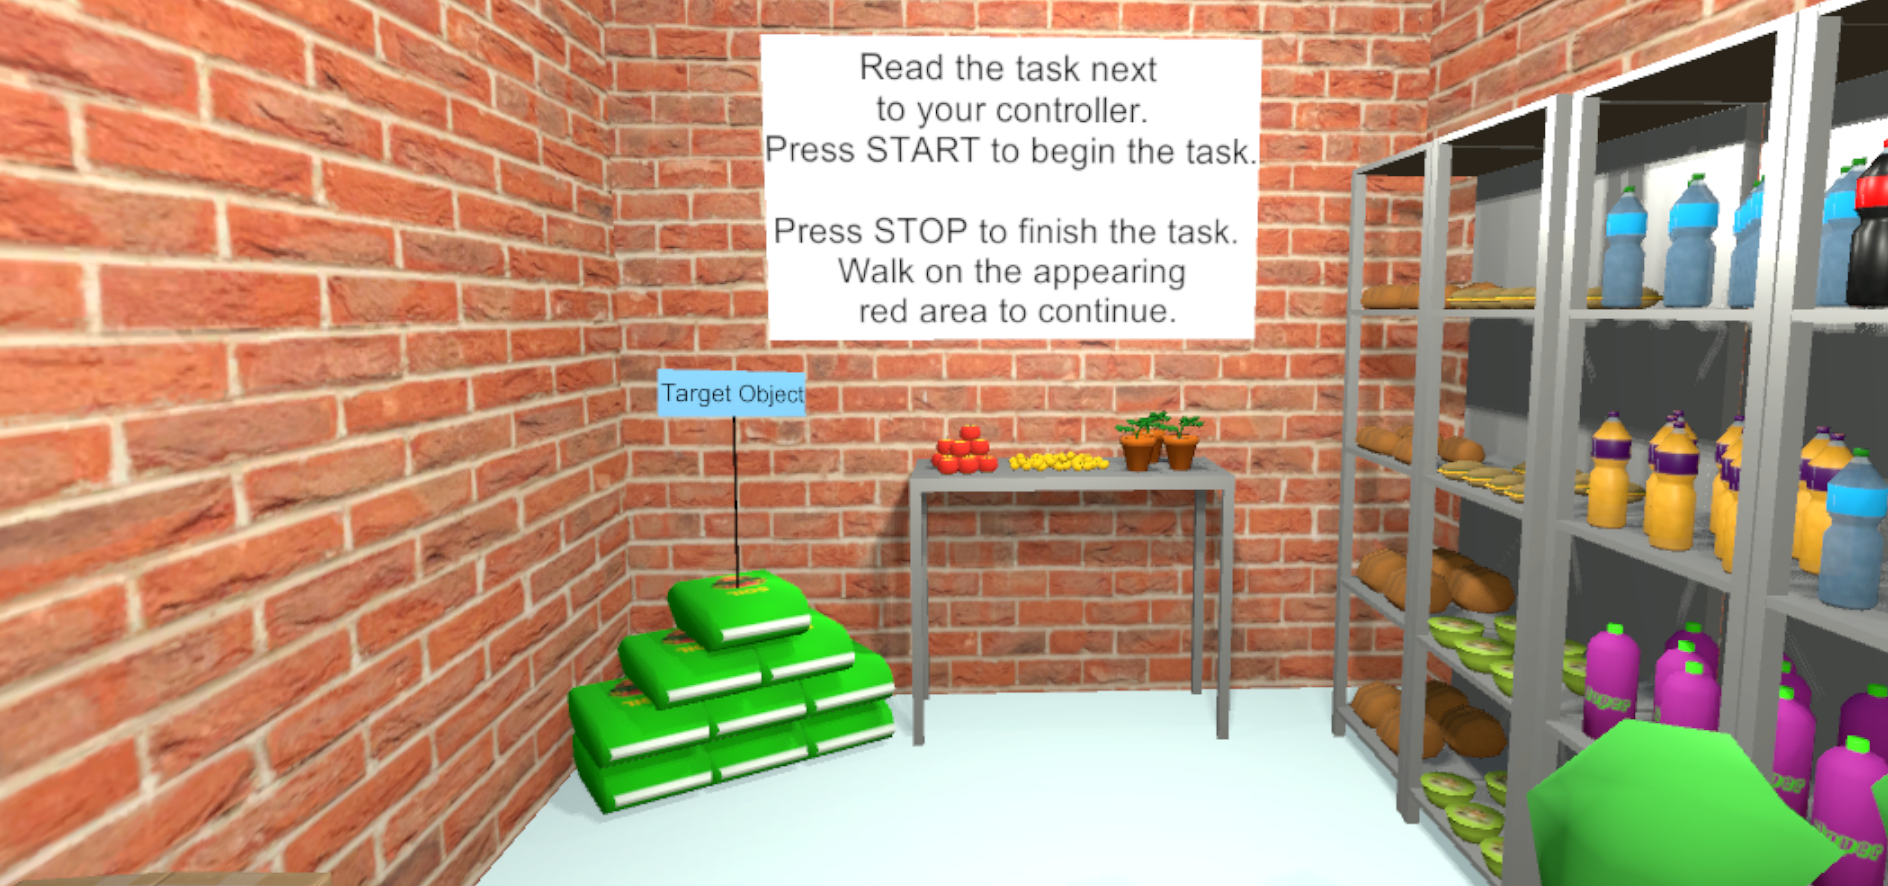
\includegraphics[width=12cm]{Images/TaskWall_1.PNG}
	\caption[Additional informations on the wall]{Additional informations on the wall}
	\label{fig:taskW1}
\end{figure}

To give the user some more information a information board within the supermarket is established, see figure \ref{fig:taskW1}. In the first tasks there are only shown some basic informations.\\
The last tasks will be repeated with every available method. That means, that the user has to pick up the same object five times. This object is so placed that the user could use close as well as far range methods. The methods are fix implemented, in order like in table \ref{tab: OrderMethods}. The methods will already  be activated as soon as the user presses start. \\

\begin{table}[h]
\centering
 \begin{tabular}{|c|c|}
  Number of subtask & Method  \\ \hline
  1 & Close Range: Touch Grab  \\
  2 & Close Range: Wand Grab  \\
  3 & Far Range: Extendable Ray  \\
  4 & Close Range: Proximity Grab  \\
  5 & Far Range: Raycast \\
   \end{tabular}
  \caption[Order of methods in the last task]{Order of methods in the last task}
	\label{tab: OrderMethods}
 \end{table}

To help the user to figure out what method will be activated the name of the method will be shown on the information board as soon as  he/she is in the new scene, like in the following figure. 

\begin{figure}[H] 
	\center 
	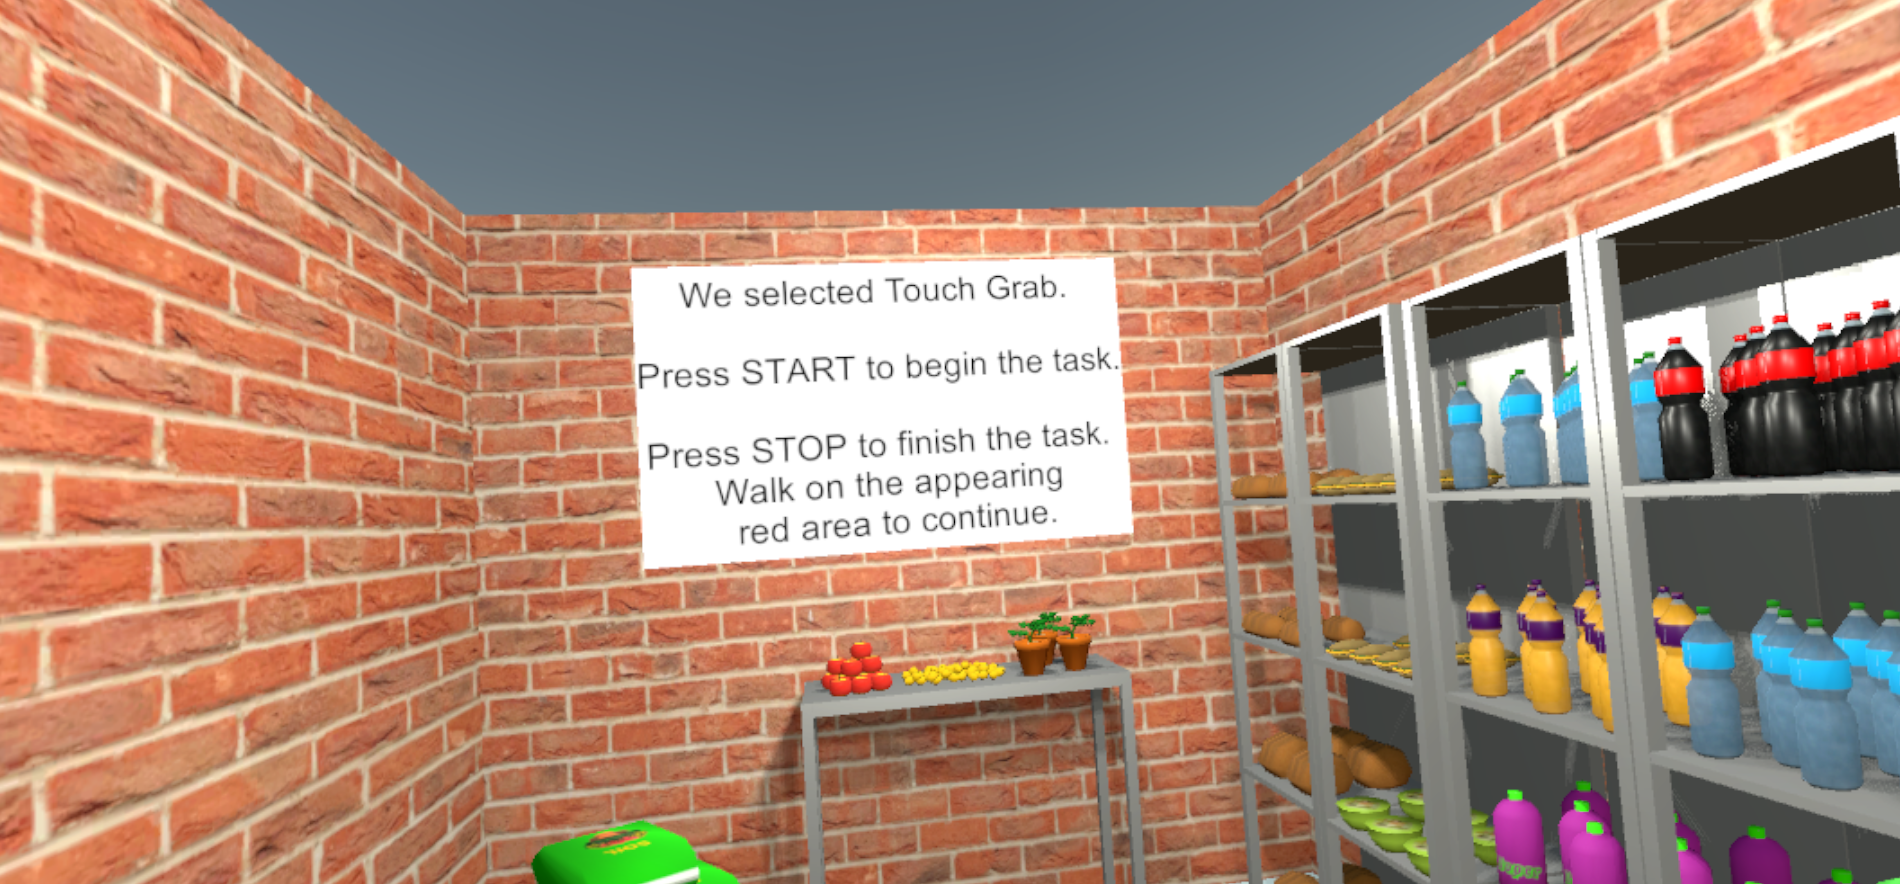
\includegraphics[width=12cm]{Images/TaskWall_2.PNG}
	\caption[Touch grab is activated]{Touch grab is activated}
	\label{fig:taskW2}
\end{figure}

In the last tasks the user has to answer an usability questionnaire about this interaction after every method. Afterwards he/she does the tasks with the next method. \\

\subsection{Measurement} \label{sec:measurement}
\todo[inline, color=red]{Vera}



\newpage